\documentclass{article}
\usepackage{microtype}
\usepackage{graphicx}
\usepackage{subfigure}
\usepackage{booktabs}
\usepackage{hyperref}

\newcommand{\theHalgorithm}{\arabic{algorithm}}

\usepackage[accepted]{icml2021}

\begin{document}

\twocolumn[
\icmltitle{RL Project: Autonomous Driving}

\icmlsetsymbol{equal}{*}

\begin{icmlauthorlist}
\icmlauthor{Michele Sprocatti}{}
\end{icmlauthorlist}


\vskip 0.3in]

\begin{abstract}
This project investigates the possibility of using a reinforcement learning agent to avoid crashes in the given highway environment \cite{highway-env}. This project compares the output of the best RL agent found with a specific baseline and with the human controlling the car. The baseline explained in Section \ref{section:Baseline} is defined in order to be an informed guess of the action that must be taken. To find the best RL agent, three different approaches are investigated: Double Deep Q-Network (DQN), Dueling Deep Q-Network (DQN), and Proximal Policy Optimization (PPO). These 3 approaches are presented in Section \ref{section:Approaches}.
\end{abstract}

\section{Introduction} \label{section:Introduction}
The highway environment \cite{highway-env} is a simple environment where we can have a variable number of lanes and different number of vehicles. The objective is to give commands to the ego vehicle (the one that is controlled) to avoid crashes and maximize rewards. The rewards are completely controlled by the environment and are normalized between -1 (crash) and 1. Each episode has a maximum duration that is set when the environment is created, so each episode can be truncated if it reaches the maximum duration or it ends with a crash.

\section{Baseline}\label{section:Baseline}
In order to define a good baseline, it was necessary to understand the information provided by the environment \cite{highway-env} through the state. In the documentation, it is explained that the specific environment (highway) uses the kinematics observation format, so in the first row, it gives the absolute information about the ego vehicle while the other rows contain the relative information of the other cars with respect to the ego vehicle.
The baseline provided uses two specific epsilons (one for the x-axis and one for the y-axis) to understand if there is a car in front of the ego vehicle. If this is true, then it moves up (if the action is available); otherwise, it moves down. If there is no vehicle in front of the ego one, the returned action will be 'FASTER'.
This baseline is not good in all cases because it does not check if there are vehicles above or below the ego one when it changes lanes, and also, with the default settings, sometimes it does not have the most updated state (since the simulation is always running), so it may crash sometimes.

\section{Approaches for RL agent} \label{section:Approaches}
To define a RL agent, 3 different approaches are explored:
\begin{itemize}
    \item Double Deep Q-Network (DQN) \cite{DoubleDeepQNetwork}
    \item Dueling Deep Q-Network (DQN) \cite{DuelDeepQNetwork}
    \item Proximal Policy Optimization (PPO) \cite{PPO}
\end{itemize}
All models were tried with different combinations of the hyperparameters in order to find the best performing one.
The three models are three deep RL approaches of increasing complexity; the first one is the simplest one of them, which is Double DQN, and then the Dueling DQN approach is explored. In the end, the state-of-the-art algorithm, the PPO, is run. The DQN base algorithm is not considered because of the problem of overestimating the function approximation.

\subsection{Double Deep-Q-Network} \label{subsection:Double}
In this approach, we have two networks ($Q$ and $Q'$) and they are used as follows: $Q$ is used to make the prediction, and in order to update it, we minimize the mean squared error between the output and the target that is built as follows:
\begin{equation}\label{eq:target_computation}
    Q^*(s_t,a_t) = R_t + \gamma * Q'(s, argmax_a Q(s_{t+1},a))
\end{equation}
For an in-depth explanation of the algorithm, look at \cite{DoubleDeepQNetwork}.

\subsection{Dueling Deep-Q-Network} \label{subsection:Duel}
In the Dueling Deep-Q-Network approach, we have two networks, but instead of predicting the Q value, each one of them has two different outputs $V(s)$ and $A(s,a)$ for every $a$ (see figure \ref{fig:duel_comparison_vanilla}), and they compute the value of $Q(s,a)$ as follows:
\begin{equation} \label{eq:q_v_a}
    Q(s,a) = V(s) + [A(s,a) + \frac{1}{|A|} *  \sum_{a'} A(s, a')]
\end{equation}
Then the target is computed similarly to the Double Deep-Q-Network; see Equation \ref{eq:target_computation}. For an in-depth explanation of the algorithm, look at \cite{DuelDeepQNetwork}.

\begin{figure}
    \centering
    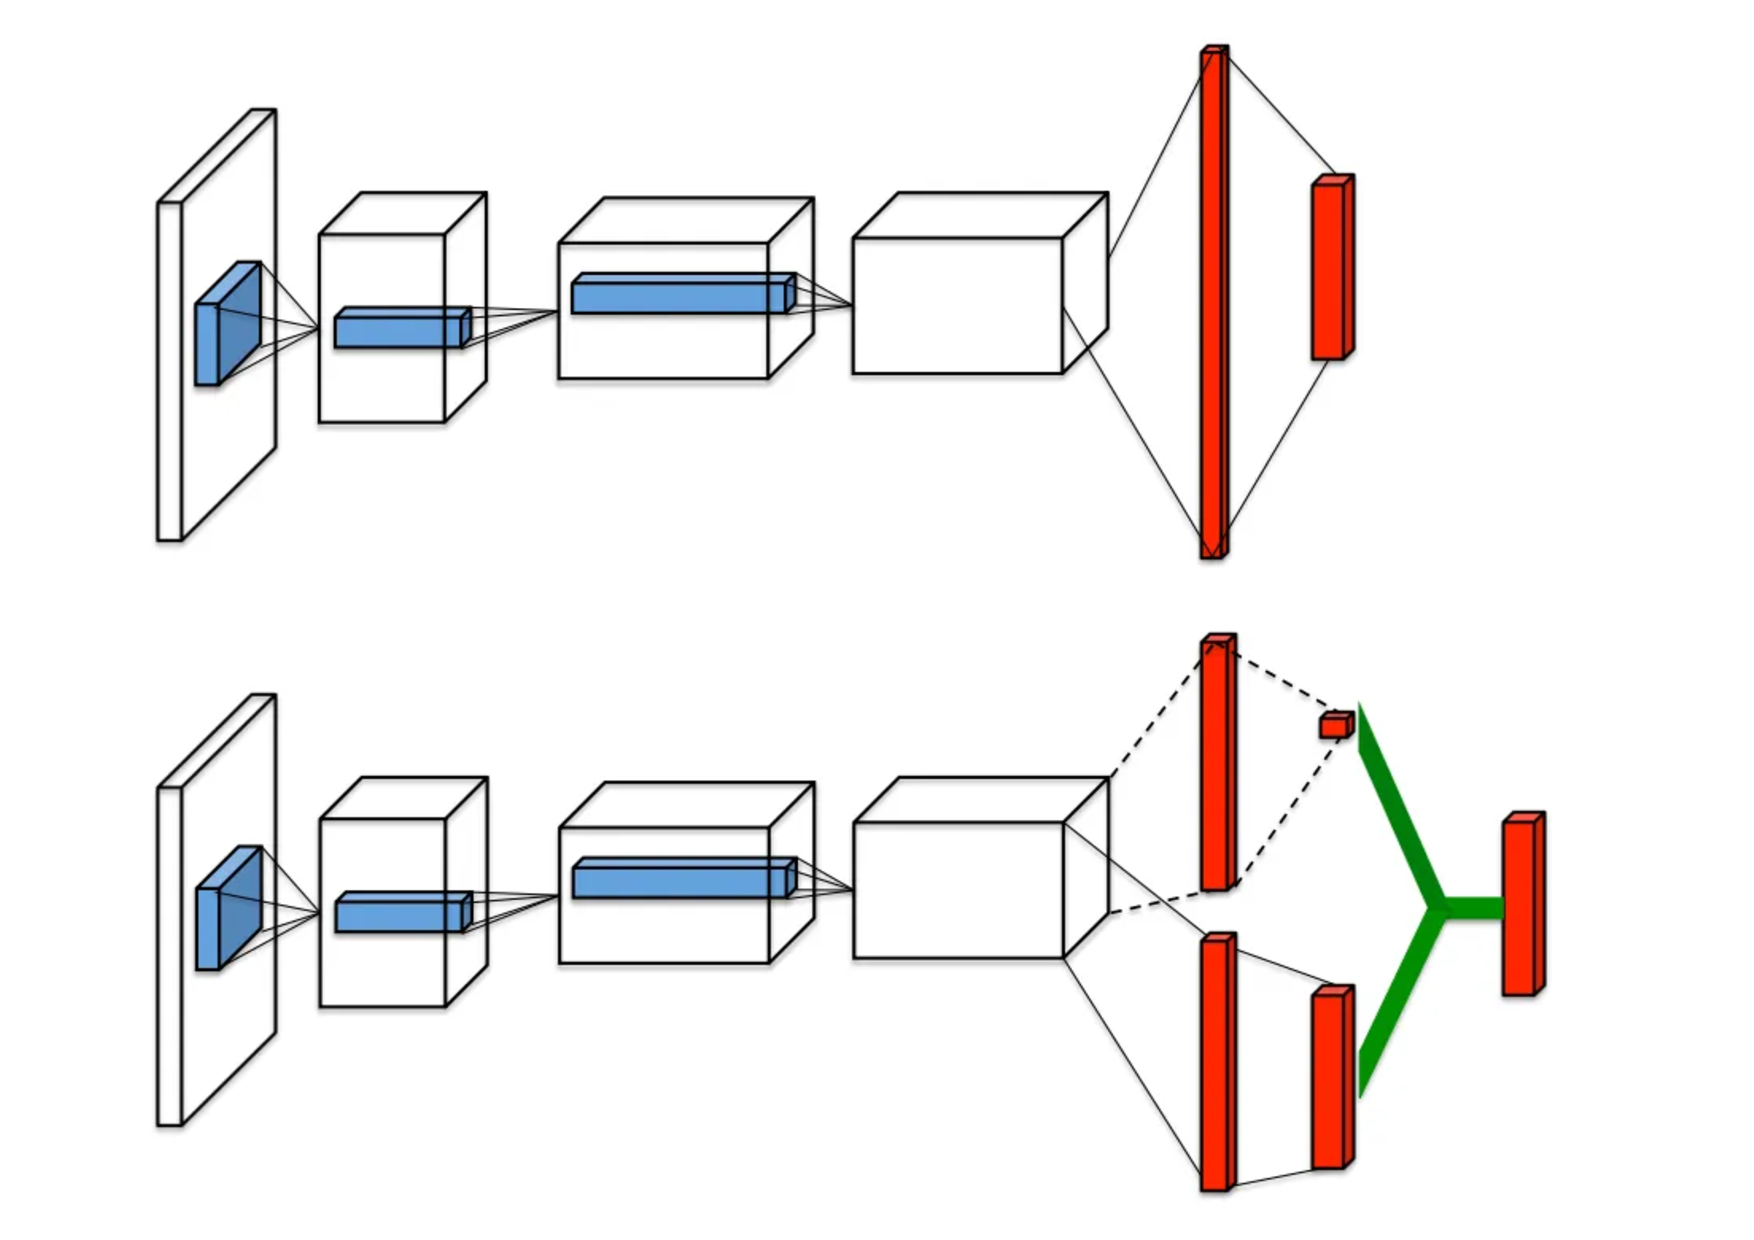
\includegraphics[width=0.7\linewidth]{img/duel_image.pdf}
    \caption{Extracted from original paper \cite{DuelDeepQNetwork} \\ Top: Regular DQN architecture. Bottom: Dueling DQN architecture.}
    \label{fig:duel_comparison_vanilla}
\end{figure}

\subsection{Proximal Policy Optimization}
The Proximal Policy Optimization is an approximation of the Trust Region Policy Optimization (TRPO) \cite{TRPO} method that enforces a trust region with the computation of the Hessian matrix; the PPO, instead, avoids the case of going out of the trust region by using a min operator and a clipping operation.
\begin{equation}
    J(\theta) = E_t [min(r_t(\theta) * A_t, clip(r_t(\theta), 1 - \epsilon, 1 + \epsilon) * A_t]
\end{equation}
Where $r_t(\theta)$ indicates the importance sampling ratio. For an in-depth explanation of the algorithm, look at \cite{PPO}.

\section{Training}\label{section:Training}
The models were trained over 4000 episodes, and from that experience, the batches of (state, action, reward, next\_state) are sampled to train the models. So, given the specific algorithm, the corresponding loss is computed, and then it is backpropagated in order to update the weights of the neural network.
Since the Double DQN and the Dueling DQN use the experience replay, the batches are sampled over all possible data, while since the PPO is an on-policy method, the data are discarded after the finish of each episode.
The outputs of the different trainings are presented in figures \ref{fig:DQN_reward_training}, \ref{fig:Duel_DQN_reward_training}, \ref{fig:PPO_reward_training}. These figures are created by plotting the average reward that the model gets for each of the 4000 episodes of the training.
Since the plots are very dense, some other plots are presented to understand how the different models improve during training. An evaluation of the model every 250 episodes of the training is carried out. The evaluation involves running 20 episodes of the model in a new environment for the current model. Then, the plot of the average return and also the average reward of these evaluation steps can be seen in figures \ref{fig:DQN_eval_return_training}, \ref{fig:DQN_eval_reward_training}, \ref{fig:Duel_DQN_eval_reward_training}, \ref{fig:DuelDQN_eval_return_training}, \ref{fig:PPO_eval_return_training}, \ref{fig:PPO_eval_reward_training}.
From these figures, it seems that the Dueling DQN algorithm and the Double DQN are the ones that learn the most because of a continuous increase in the average return, while the PPO is more oscillating between low and high returns. From the plot of the average reward, it can be seen that the PPO does not change a lot during the training, while the Double DQN and the Dueling DQN seems to learn a lot, but the Dueling DQN reaches a better average reward in the end.

\begin{figure}
    \centering
    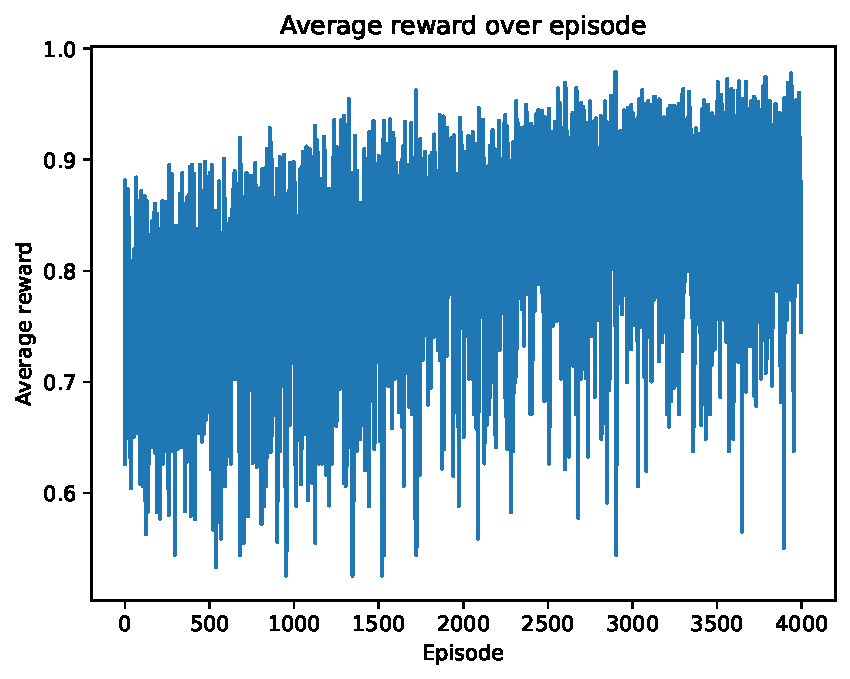
\includegraphics[width=0.7\linewidth]{img/DQN_training.pdf}
    \caption{Double DQN training average reward}
    \label{fig:DQN_reward_training}
\end{figure}

\begin{figure}
    \centering
    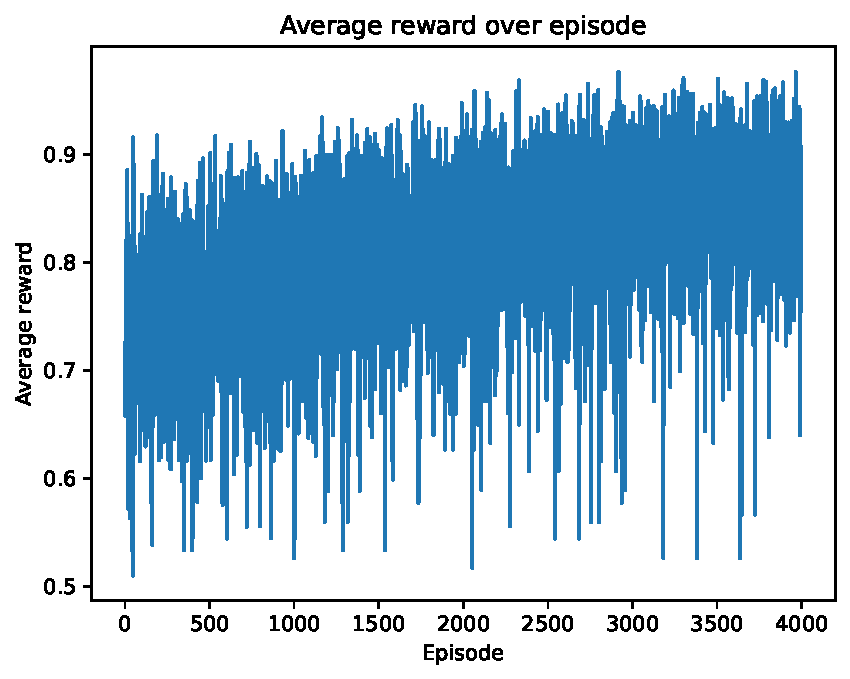
\includegraphics[width=0.7\linewidth]{img/DuelDQN_training.pdf}
    \caption{Dueling DQN training average reward}
    \label{fig:Duel_DQN_reward_training}
\end{figure}

\begin{figure}
    \centering
    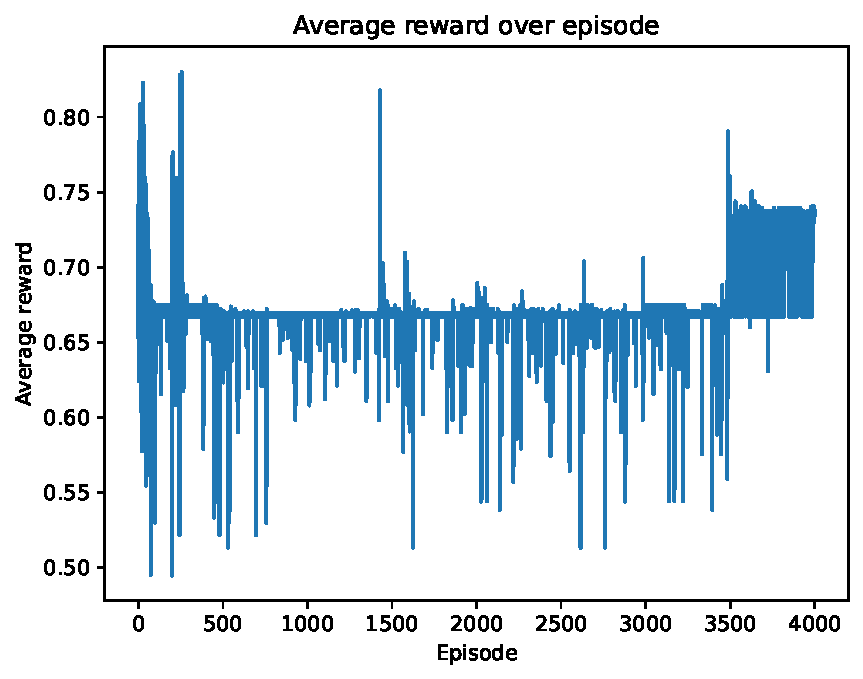
\includegraphics[width=0.7\linewidth]{img/PPO_training.pdf}
    \caption{PPO training average reward}
    \label{fig:PPO_reward_training}
\end{figure}

\begin{figure}
    \centering
    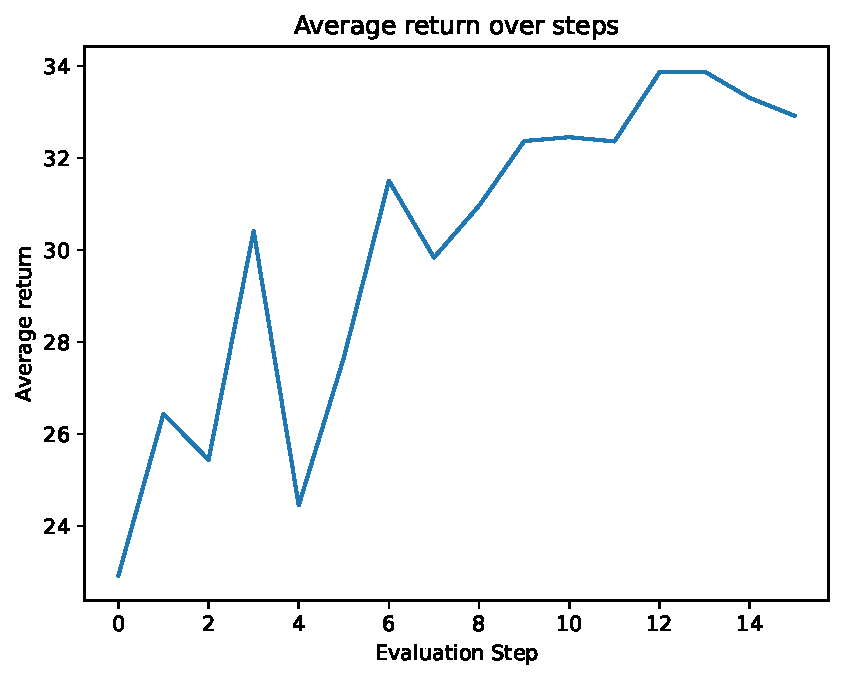
\includegraphics[width=0.7\linewidth]{img/DQN_training_eval_return.pdf}
    \caption{Double DQN training evaluation return}
    \label{fig:DQN_eval_return_training}
\end{figure}

\begin{figure}
    \centering
    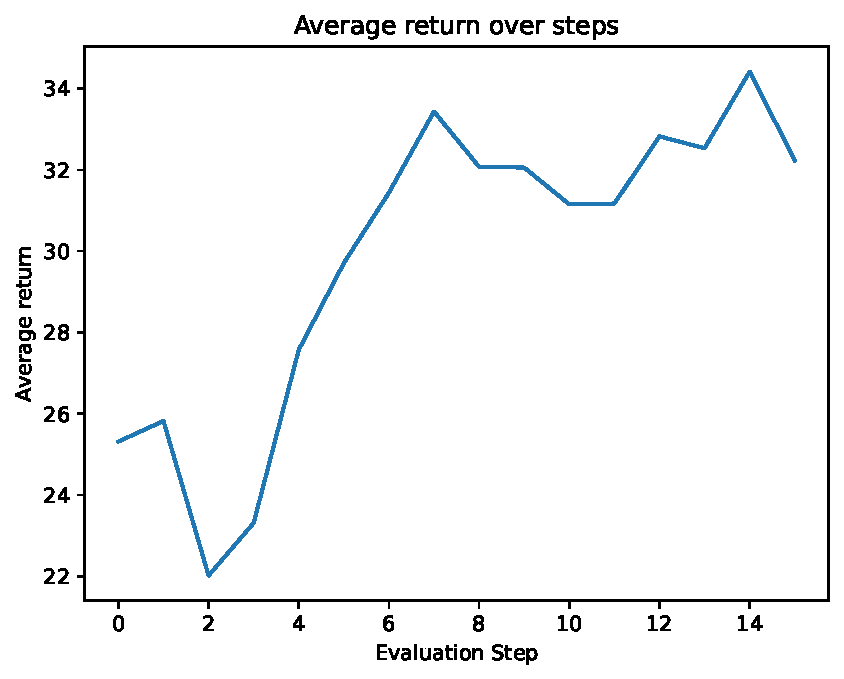
\includegraphics[width=0.7\linewidth]{img/DuelDQN_training_eval_return.pdf}
    \caption{Dueling DQN training evaluation return}
    \label{fig:DuelDQN_eval_return_training}
\end{figure}

\begin{figure}
    \centering
    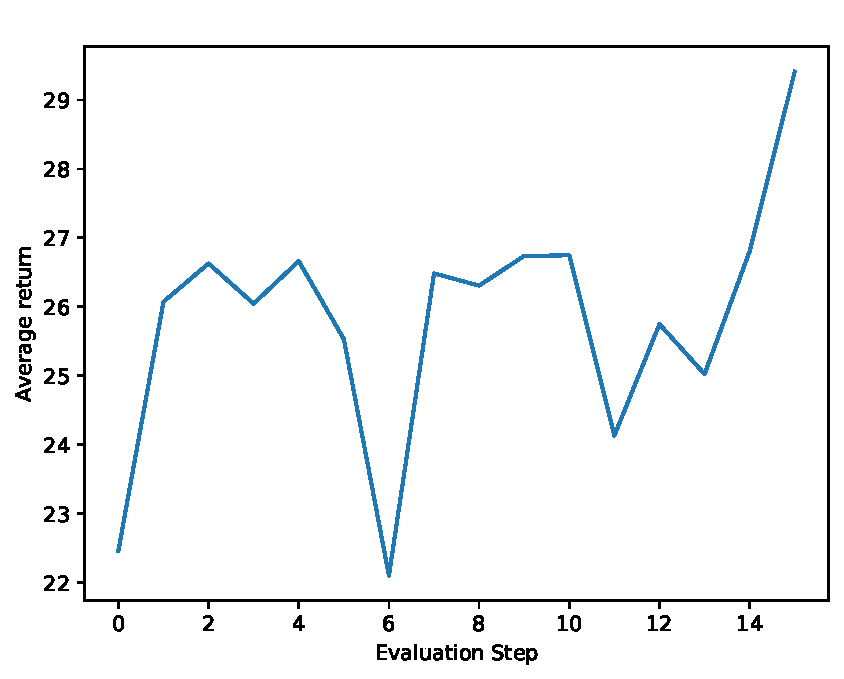
\includegraphics[width=0.7\linewidth]{img/PPO_training_eval_return.pdf}
    \caption{PPO training evaluation return}
    \label{fig:PPO_eval_return_training}
\end{figure}

\begin{figure}
    \centering
    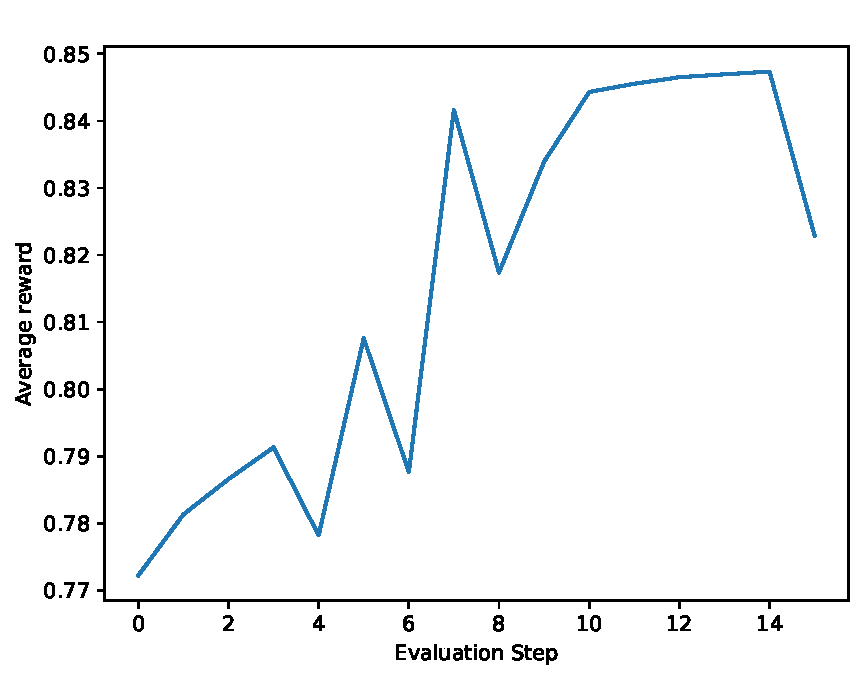
\includegraphics[width=0.7\linewidth]{img/DQN_training_eval_avg_reward.pdf}
    \caption{Double DQN training evaluation average reward}
    \label{fig:DQN_eval_reward_training}
\end{figure}

\begin{figure}
    \centering
    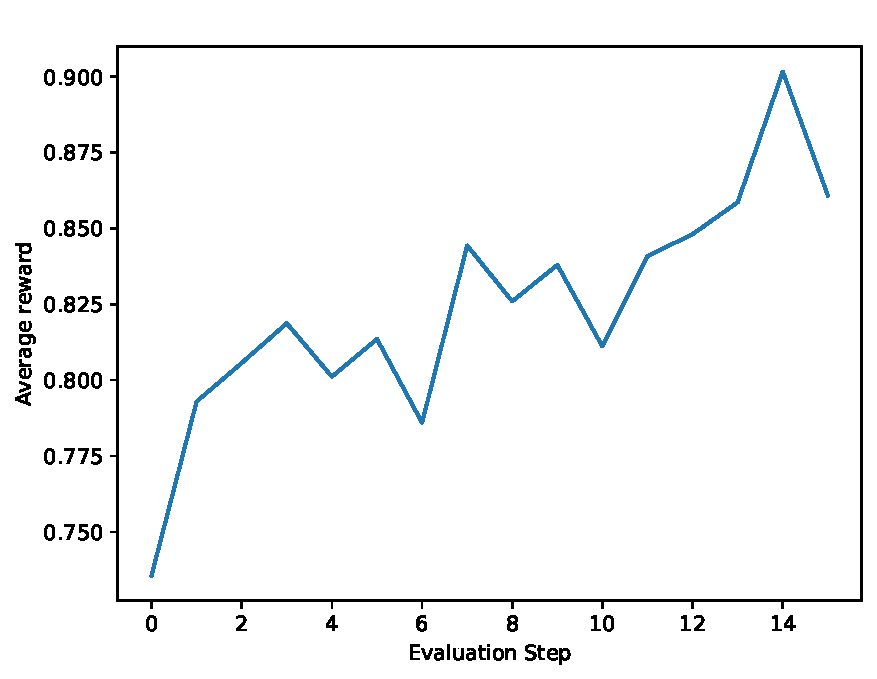
\includegraphics[width=0.7\linewidth]{img/DuelDQN_training_eval_avg_reward.pdf}
    \caption{Dueling DQN training evaluation average reward}
    \label{fig:Duel_DQN_eval_reward_training}
\end{figure}

\begin{figure}
    \centering
    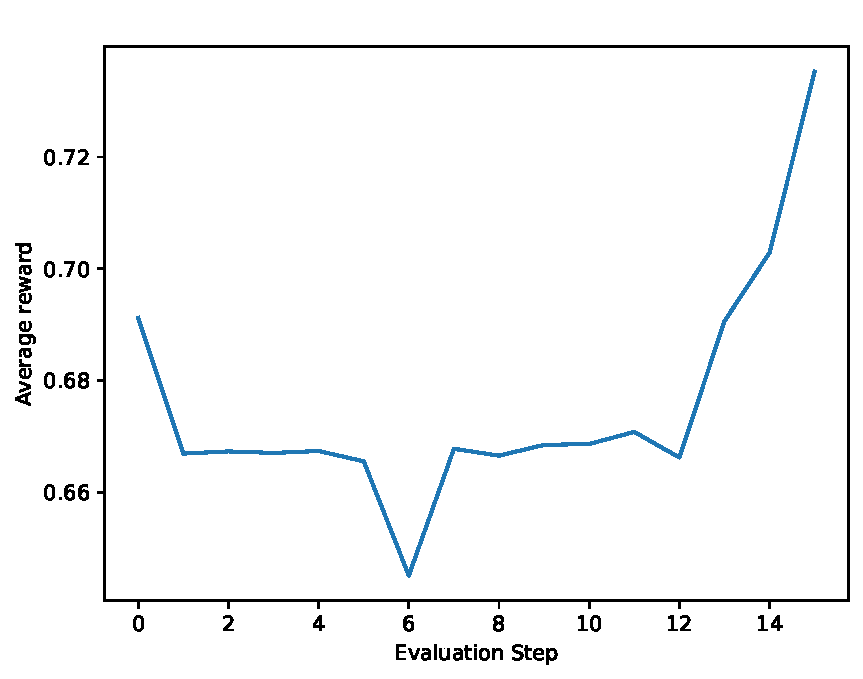
\includegraphics[width=0.7\linewidth]{img/PPO_training_eval_avg_reward.pdf}
    \caption{PPO training evaluation average reward}
    \label{fig:PPO_eval_reward_training}
\end{figure}

\section{Results}\label{section:Results}
The results are obtained by evaluating the different models on the environment and comparing them with the manual control and the specific baseline. The return and the average reward with manual control can be seen in figures \ref{fig:Return_episode_manual} and \ref{fig:Reward_episode_manual}. These are very high since the human can avoid crashes in a very good way.
The baseline output can be seen in figures \ref{fig:Return_episode_baseline} and \ref{fig:Reward_episode_baseline} . From these figures, we can see that the baseline is good when it comes to selecting the action because we have a very high average reward, and this comes from the fact that in the general case it returns 'FASTER', but it does not avoid all crashes because when it changes lanes it does not check if the others are free, and also some crashes happen because it sees the vehicle in front too late, and this causes the returns to not be very high.
For the three reinforcement learning agents, we can see the results in figures \ref{fig:Return_episode_DQN}, \ref{fig:Reward_episode_DQN}, \ref{fig:Return_episode_Duel_DQN}, \ref{fig:Reward_episode_Duel_DQN}, \ref{fig:Return_episode_PPO}, \ref{fig:Reward_episode_PPO}. From these plots, we can see that the Dueling DQN algorithm provided the best model because it has the highest reward on average with also more stability and very high returns over the different episodes. The Double DQN has a very high return, but the average reward is less stable and oscillates a lot between low and high values, while the PPO has lower returns because it moves the ego vehicle in the rightmost lane and then stays there but avoids crashes by selecting 'SLOWER'.
By comparing the Dueling DQN that seems to be the best reinforcement learning agent and the baseline, we can see that the agent performs better because it obtains a higher return thanks to the fact that the episode lasts longer, but also it obtains higher average reward. Obviously, the human-controlled one seems to be the best, but the Dueling DQN agent reaches very similar performance in terms of rewards and returns.

\begin{figure}
    \centering
    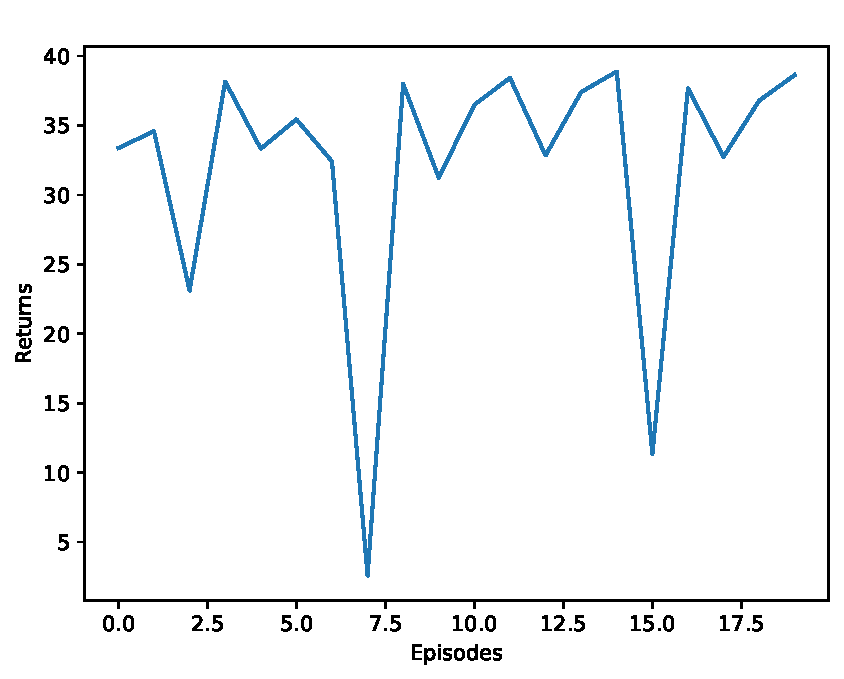
\includegraphics[width=0.7\linewidth]{img/Return_over_episode_manual.pdf}
    \caption{Return over the episode with manual control}
    \label{fig:Return_episode_manual}
\end{figure}

\begin{figure}
    \centering
    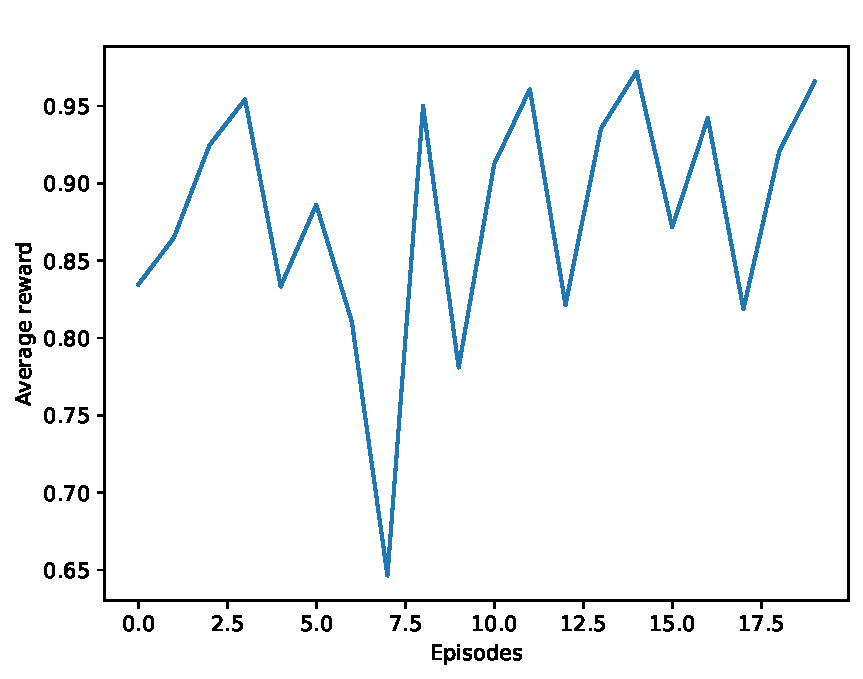
\includegraphics[width=0.7\linewidth]{img/Average_reward_over_episode_manual.pdf}
    \caption{Average reward over the episode with manual control}
    \label{fig:Reward_episode_manual}
\end{figure}

\begin{figure}
    \centering
    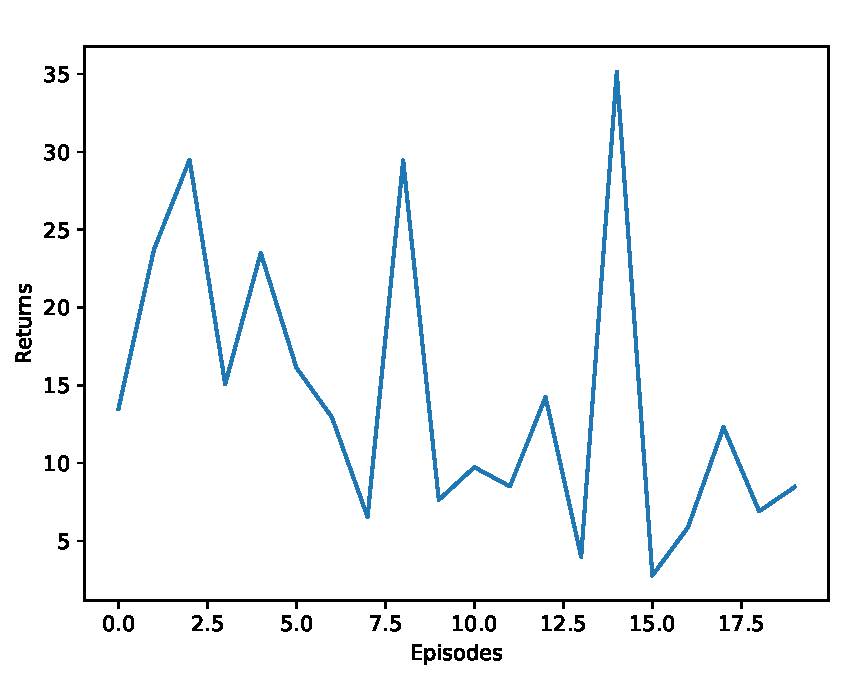
\includegraphics[width=0.7\linewidth]{img/Return_over_episode_baseline.pdf}
    \caption{Return over episode baseline}
    \label{fig:Return_episode_baseline}
\end{figure}

\begin{figure}
    \centering
    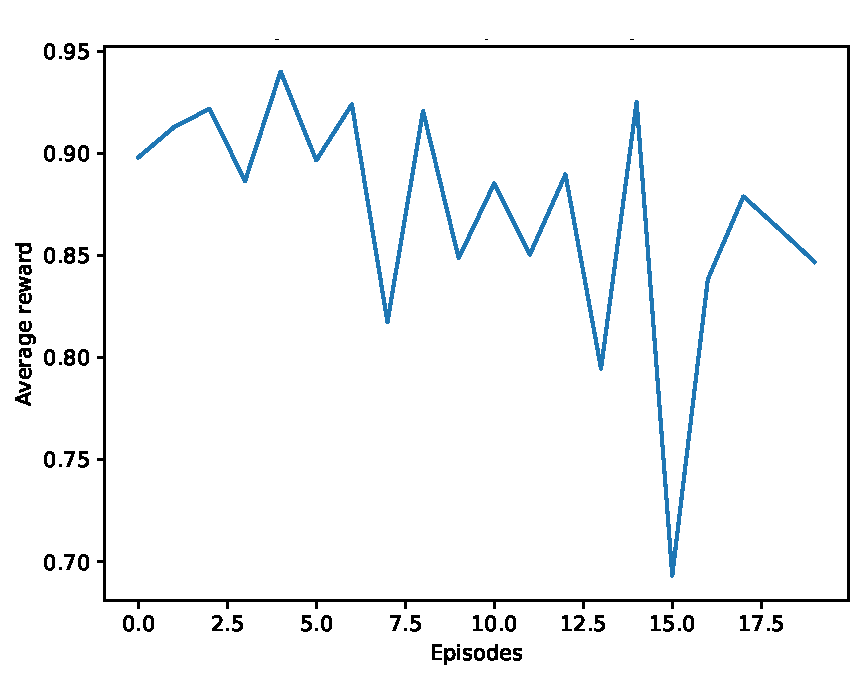
\includegraphics[width=0.7\linewidth]{img/Average_reward_over_episode_baseline.pdf}
    \caption{Average reward over episode baseline}
    \label{fig:Reward_episode_baseline}
\end{figure}

\begin{figure}
    \centering
    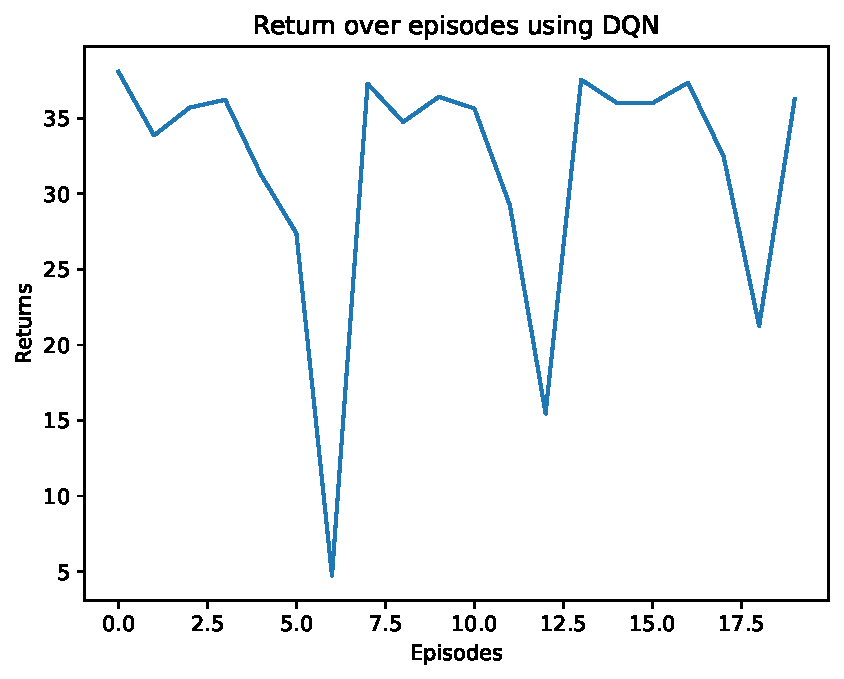
\includegraphics[width=0.7\linewidth]{img/Return_over_episode_DQN_4000.pdf}
    \caption{Return over episode DQN}
    \label{fig:Return_episode_DQN}
\end{figure}

\begin{figure}
    \centering
    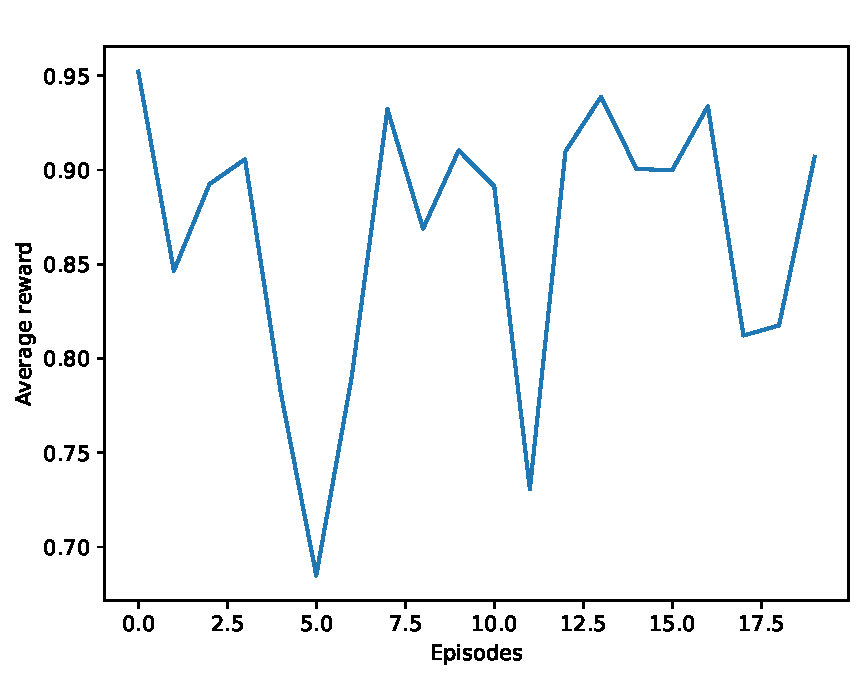
\includegraphics[width=0.7\linewidth]{img/Average_reward_over_episode_DQN_4000.pdf}
    \caption{Average reward over episode DQN}
    \label{fig:Reward_episode_DQN}
\end{figure}

\begin{figure}
    \centering
    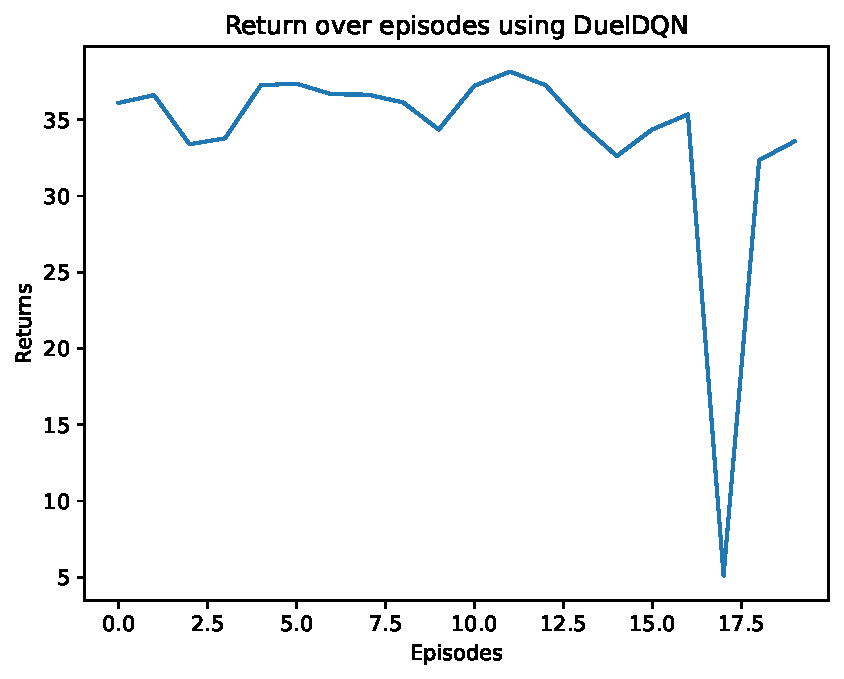
\includegraphics[width=0.7\linewidth]{img/Return_over_episode_DuelDQN_4000.pdf}
    \caption{Return over episode Dueling DQN}
    \label{fig:Return_episode_Duel_DQN}
\end{figure}

\begin{figure}
    \centering
    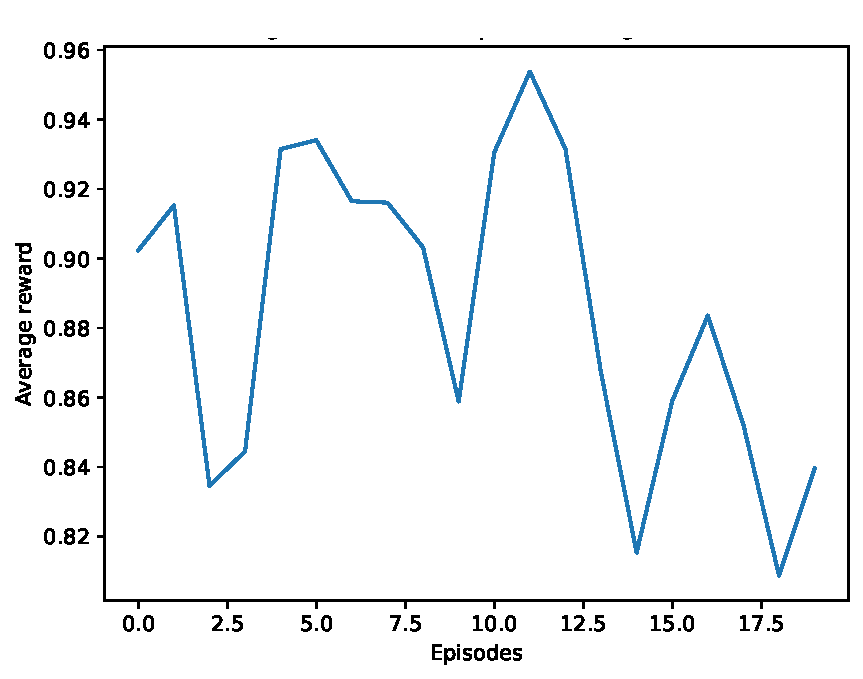
\includegraphics[width=0.7\linewidth]{img/Average_reward_over_episode_DuelDQN_4000.pdf}
    \caption{Average reward over episode Dueling DQN}
    \label{fig:Reward_episode_Duel_DQN}
\end{figure}

\begin{figure}
    \centering
    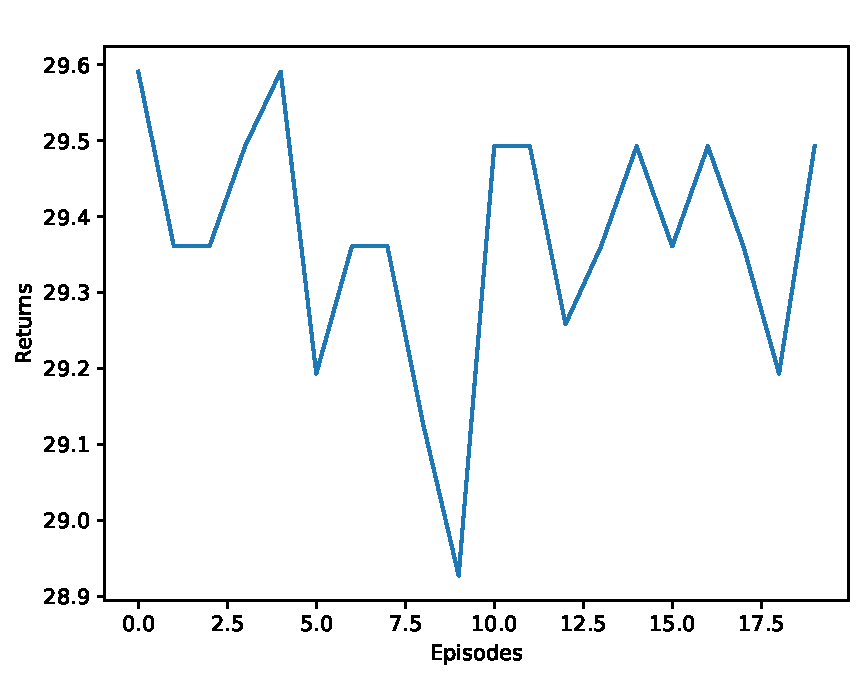
\includegraphics[width=0.7\linewidth]{img/Return_over_episode_PPO_4000.pdf}
    \caption{Return over episode PPO}
    \label{fig:Return_episode_PPO}
\end{figure}

\begin{figure}
    \centering
    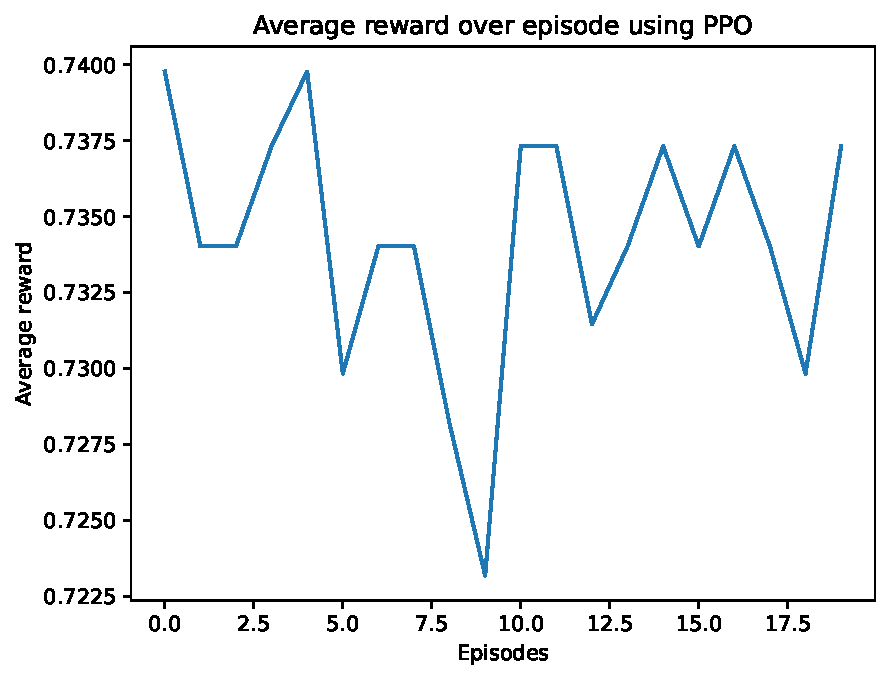
\includegraphics[width=0.7\linewidth]{img/Average_reward_over_episode_PPO_4000.pdf}
    \caption{Average reward over episode PPO}
    \label{fig:Reward_episode_PPO}
\end{figure}

\section{Conclusions} \label{section:Conclusions}
From the three approaches presented, we can see that the Double DQN and the Dueling DQN are the two that perform the best because the PPO has lower returns. Between the Double DQN and the Dueling DQN, the one that seems to work best is the Dueling DQN because it achieves higher returns and highest average rewards.
By comparing the Dueling DQN with the baseline, we can see that the the model outperformed the specific baseline in terms of returns; and it reaches similar performance compare to the human.

\bibliography{main}
\bibliographystyle{icml2021}

\end{document}